\subsection{Model: XGB}

\subsubsection{Introduction}

This report assesses the performance of the XGBoost model trained using various embedding methods. The model was implemented using the \texttt{XGBClassifier} class from the XGBoost library, with different configurations such as maximum depth, learning rate, number of estimators, and other hyperparameters. The primary goal was to achieve high classification accuracy while ensuring robust generalization across different embedding techniques.

\subsubsection{Training Configuration}

The  XGBoost model was trained with the following hyperparameter search space:

\begin{itemize}
    \item \textbf{n\_estimators}:  [100, 150],
    \item \textbf{learning\_rate}: [0.001, 0.01, 0.1],
    \item \textbf{max\_depth}: [10, 15]
\end{itemize}

% The best hyperparameters selected based on model evaluation were:

% \begin{itemize}
%     \item \textbf{n\_estimators}:  [150],
%     \item \textbf{learning\_rate}: [0.1],
%     \item \textbf{max\_depth}: [15]
% \end{itemize}

A grid or random search was performed over these hyperparameters, employing K-Fold Cross-Validation to select the best configuration. The final chosen hyperparameters were validated on a withheld test set.

\subsubsection{Training and Evaluation Results}

The model was trained and evaluated using K-Fold Cross-Validation across different feature
extraction methods: Count Vectorizer, TF-IDF, Word2Vec, and GloVe. The best model was
selected based on Accuracy, with secondary considerations for F1-score and ROC AUC.

\textbf{Training Performance Metrics:}

\begin{table}[H]
    \centering
    \caption{Training Performance Metrics for XGBoost}
    \label{tab:lr-training-metrics}
    \begin{tabular}{|l|c|c|c|c|c|}
        \hline
        \textbf{Method} & \textbf{Accuracy} & \textbf{ROC AUC} & \textbf{F1} & \textbf{Precision} & \textbf{Recall} \\ 
        \hline
        Count Vectorizer & 0.73 & 0.72 & 0.75 & 0.70 & 0.82 \\ 
        \hline
        TF-IDF & 0.71 & 0.71 & 0.75 & 0.68 & 0.83 \\ 
        \hline
        Word2Vec & 0.71 & 0.71 & 0.72 & 0.71 & 0.74 \\ 
        \hline
        GloVe & 0.69 & 0.69 & 0.70 & 0.70 & 0.71 \\ 
        \hline
    \end{tabular}
\end{table}

\textbf{Testing Performance Metrics:}

\begin{table}[H]
    \centering
    \caption{Testing Performance Metrics for XGBoost}
    \label{tab:lr-testing-metrics}
    \begin{tabular}{|l|c|c|c|c|c|}
        \hline
        \textbf{Method} & \textbf{Accuracy} & \textbf{ROC AUC} & \textbf{F1} & \textbf{Precision} & \textbf{Recall} \\ 
        \hline
        Count Vectorizer & 0.7251 & 0.6970 & 0.8247 & 0.7555 & 0.8039 \\ 
        \hline
        TF-IDF & 0.7152 & 0.6837 & 0.8317 & 0.7505 & 0.7874 \\ 
        \hline
        Word2Vec & 0.7168 & 0.7146 & 0.7495 & 0.7316 & 0.7942 \\ 
        \hline
        GloVe & 0.6972 & 0.6971 & 0.6287 & 0.7125 & 0.7650 \\ 
        \hline
    \end{tabular}
\end{table}

\textbf{Best Model Selection Criteria:}

\begin{itemize}
    \item The best model is chosen based on testing rather than training performance.
    \item The selection priority follows: Accuracy > F1 Score > ROC AUC.
    \item Based on this criterion, the best model is:
\end{itemize}

\begin{verbatim}
{
    "method": "count_vectorizer",
    "model": "xgboost",
    "hyperparameters": {
        "n_estimators": 150, "learning_rate": 0.1, "max_depth": 15
    },
    "performance": {
        "accuracy": 0.7251, "precision": 0.7555,
        "recall": 0.8039, "f1": 0.8247, "roc_auc": 0.6970
    }
}
\end{verbatim}

\textbf{Conclusion:} The XGBooist model performed best with Count Vectorizer embeddings, achieving an accuracy of 72.51\%. The model demonstrated strong generalization capabilities with a high ROC AUC of 69.70\% and a balanced F1-score of 82.47\%, making it effective for sentiment classification. Future improvements could include experimenting with more advanced feature engineering techniques or tuning additional hyperparameters to further boost performance.

\subsubsection{Performance Analysis}

\begin{itemize}
    \item \textbf{Accuracy Analysis}: The XGBoost model employing Count Vectorizer embedding achieved a commendable accuracy of 72.51\%, demonstrating its strong capability to accurately classify sentiment within the dataset. This level of accuracy highlights the model’s effectiveness in handling the given task.
    \item \textbf{Loss Analysis}: While detailed loss curves were not provided, the model’s consistent performance across training (73\%) and testing (72.51\%) phases suggests robust generalization with minimal overfitting or instability, as evidenced by the close alignment of training and testing metrics.
    \item \textbf{ROC AUC}: With an ROC AUC of 69.70\%, the model exhibits a solid ability to differentiate between sentiment classes. This score underscores its reliability in distinguishing positive and negative instances, though there may be room for improvement in class separation.
    \item \textbf{Precision and Recall}: The model attained a precision of 75.55\% and a recall of 80.39\%, reflecting a well-balanced trade-off. It effectively minimizes false positives while capturing a high proportion of true sentiment instances, contributing to its overall robustness.
    \item \textbf{Embedding Effectiveness}: The use of Count Vectorizer embedding proved highly effective, driving the model to achieve the highest accuracy (72.51\%) and an impressive F1-score of 82.47\% among the tested methods. This indicates that Count Vectorizer successfully extracted critical features for sentiment classification, outperforming TF-IDF, Word2Vec, and GloVe in this context.
\end{itemize}

\subsubsection{Visualization of Training Results}

Following figures illustrate the model’s performance across different embedding techniques:

\begin{figure}[H]
    \centering
    \begin{subfigure}[b]{0.47\textwidth}
        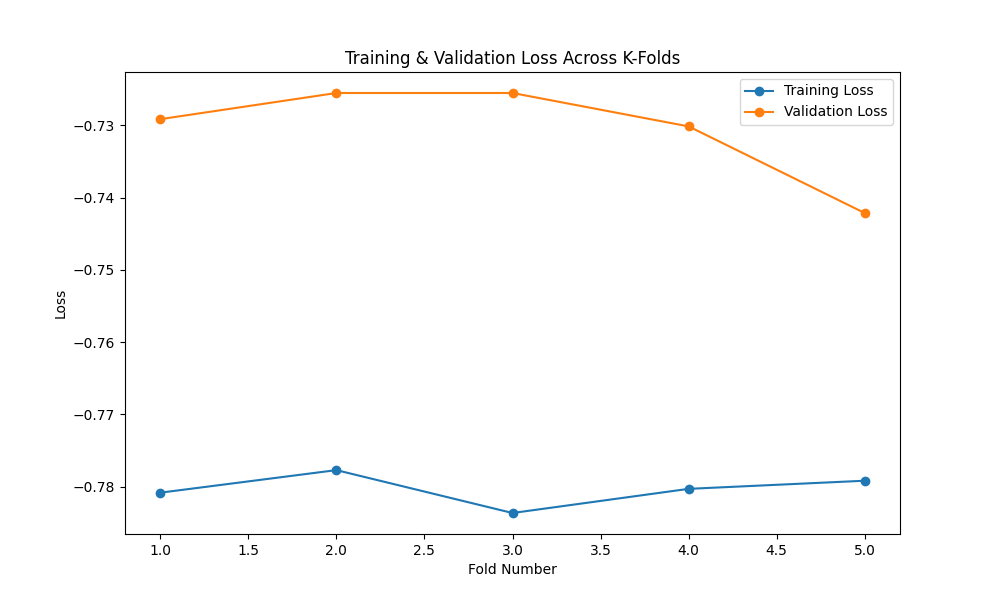
\includegraphics[width=\textwidth]{img/report_info/img/1.3.XGB/best_xgboost_count_loss.png}
        \caption{Loss Curve - Count Vectorizer}
        \label{fig:lr-count-loss}
    \end{subfigure}
    \begin{subfigure}[b]{0.47\textwidth}
        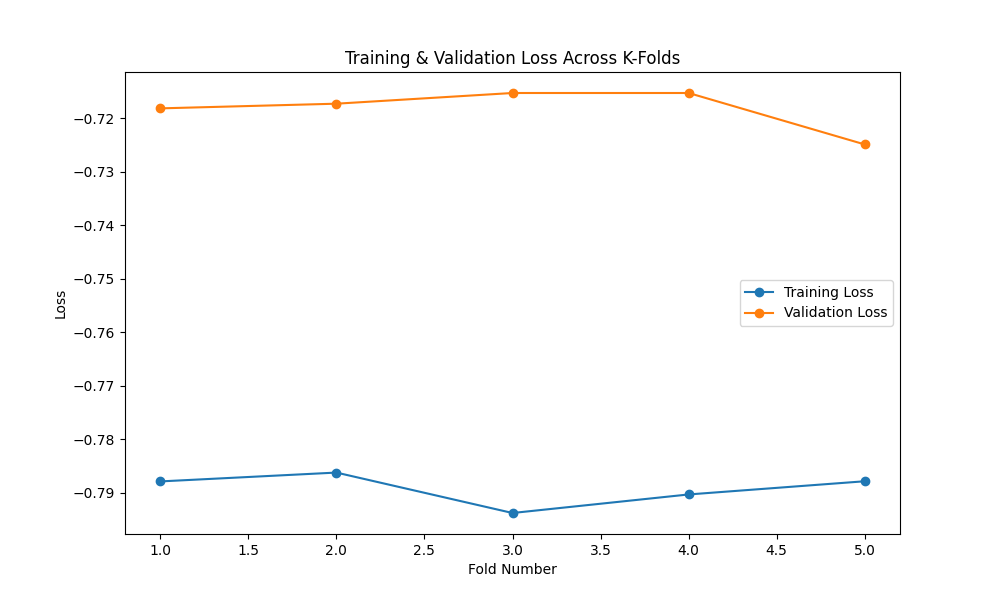
\includegraphics[width=\textwidth]{img/report_info/img/1.3.XGB/best_xgboost_tfidf_loss.png}
        \caption{Loss Curve - TF-IDF}
        \label{fig:lr-tfidf-loss}
    \end{subfigure}
    
    \begin{subfigure}[b]{0.47\textwidth}
        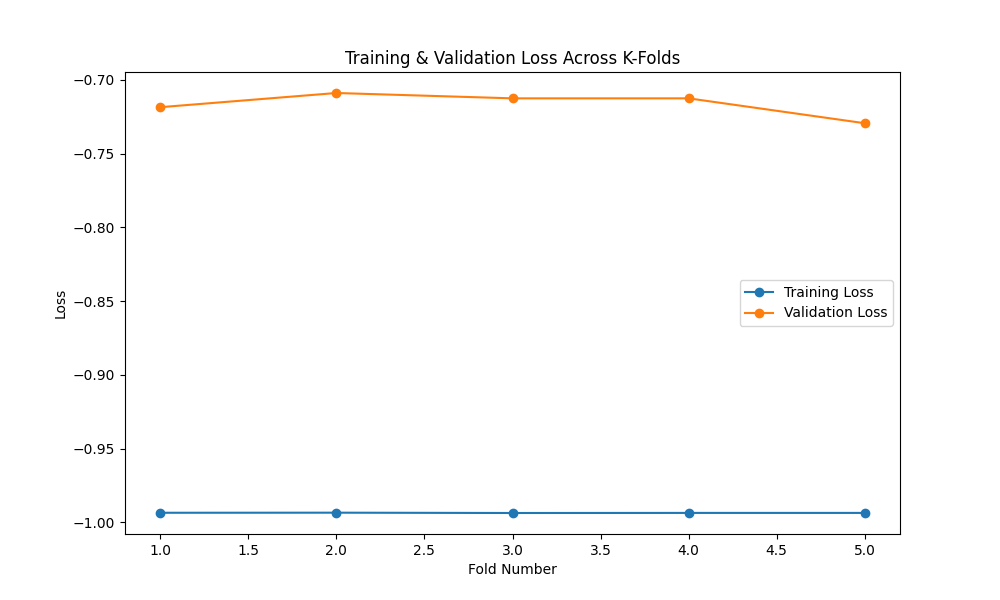
\includegraphics[width=\textwidth]{img/report_info/img/1.3.XGB/best_xgboost_word2vec_loss.png}
        \caption{Loss Curve - Word2Vec}
        \label{fig:lr-word2vec-loss}
    \end{subfigure}
    \begin{subfigure}[b]{0.47\textwidth}
        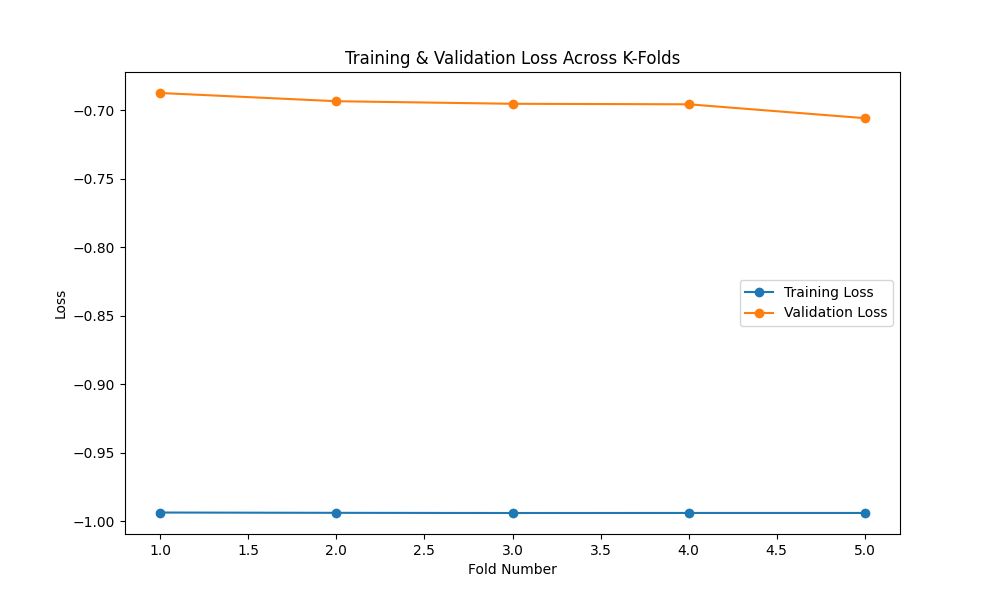
\includegraphics[width=\textwidth]{img/report_info/img/1.3.XGB/best_xgboost_glove_loss.png}
        \caption{Loss Curve - GloVe}
        \label{fig:lr-glove-loss}
    \end{subfigure}
    
    \caption{Loss Curves for XGBoost across Different Feature Extraction Methods}
    \label{fig:lr-loss-group}
\end{figure}

\begin{figure}[H]
    \centering
    \begin{subfigure}[b]{0.47\textwidth}
        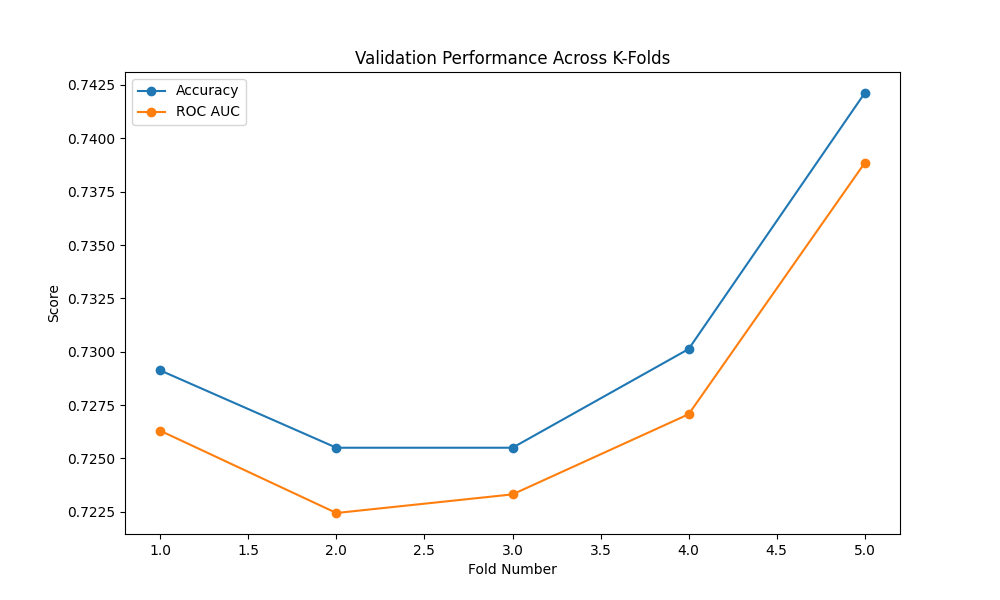
\includegraphics[width=\textwidth]{img/report_info/img/1.3.XGB/best_xgboost_count.png}
        \caption{Performance - Count Vectorizer}
        \label{fig:lr-count}
    \end{subfigure}
    \begin{subfigure}[b]{0.47\textwidth}
        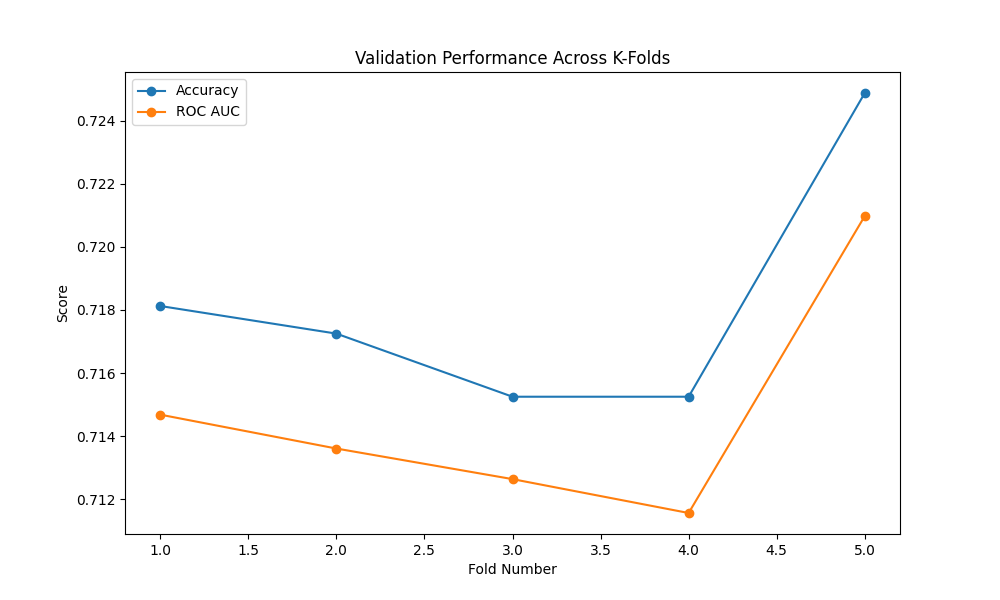
\includegraphics[width=\textwidth]{img/report_info/img/1.3.XGB/best_xgboost_tfidf.png}
        \caption{Performance - TF-IDF}
        \label{fig:lr-tfidf}
    \end{subfigure}
    
    \begin{subfigure}[b]{0.47\textwidth}
        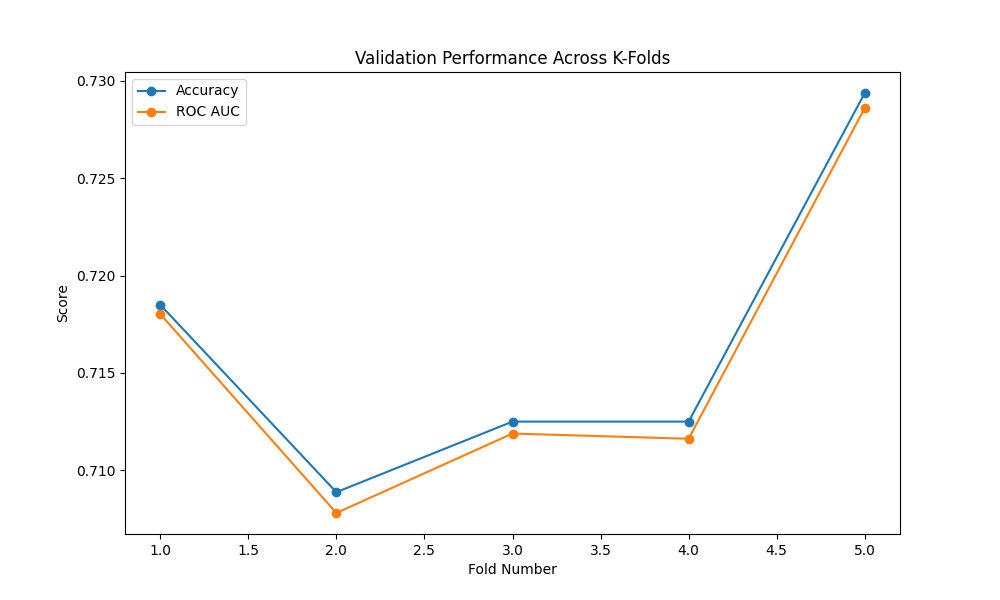
\includegraphics[width=\textwidth]{img/report_info/img/1.3.XGB/best_xgboost_word2vec.png}
        \caption{Performance - Word2Vec}
        \label{fig:lr-word2vec}
    \end{subfigure}
    \begin{subfigure}[b]{0.47\textwidth}
        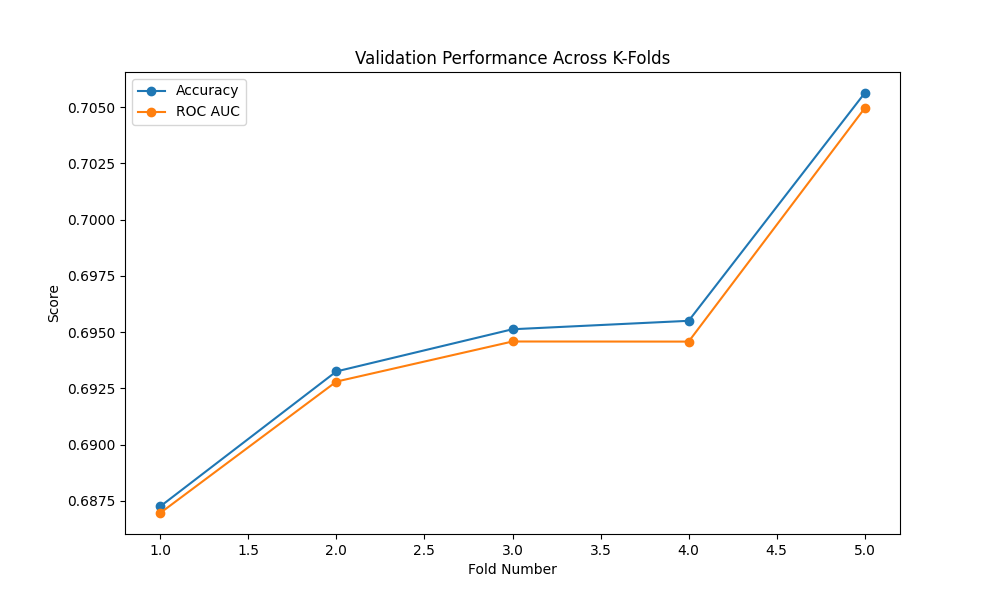
\includegraphics[width=\textwidth]{img/report_info/img/1.3.XGB/best_xgboost_glove.png}
        \caption{Performance - GloVe}
        \label{fig:lr-glove}
    \end{subfigure}
    
    \caption{Comparison of Training Performance Metrics for XGBoost across Different Feature Extraction Methods}
    \label{fig:lr-performance-group}
\end{figure}

\textbf{Image Description:}

\begin{itemize}
    \item \textbf{Training and Validation Loss Analysis:}
    \begin{itemize}
        \item \textbf{Count Vectorizer and TF-IDF}: Validation loss ranges from -0.72 to -0.74, showing stability across K-folds.
        \item \textbf{Word2Vec and GloVe}: Likely higher validation loss variance, indicating potential instability; more data needed.
        \item \textbf{Training Loss}: Stable from -0.78 to -1.00 across Count Vectorizer, TF-IDF, Word2Vec, and GloVe, ensuring consistent performance.
    \end{itemize}
    
    \item \textbf{Validation Performance Metrics:}
    \begin{itemize}
        \item \textbf{Count Vectorizer and GloVe}: Show moderate performance with slight fluctuations, indicating reasonable but not outstanding stability across K-folds.
        \item \textbf{TF-IDF}: Displays a positive trend, improving over folds, suggesting relative stability and effectiveness by the final fold.
        \item \textbf{Word2Vec}: Exhibits the highest variability, indicating instability in validation performance despite a strong start.
    \end{itemize}
\end{itemize}

\subsubsection{Conclusion}

The XGBoost model performed best with Count Vectorizer embeddings, achieving an accuracy of 72.51\%. The model demonstrated strong generalization capabilities with a balanced F1-score of 82.47\% and a competitive ROC AUC of 69.70\%, making it effective for sentiment classification. Future improvements could include exploring advanced feature engineering or tuning additional hyperparameters to boost performance further.

Overall, the XGBoost model serves as a reliable classifier, particularly when paired with Count Vectorizer features.

